\documentclass[nooutcomes]{ximera}
%\documentclass[space,handout,nooutcomes]{ximera}

% For preamble materials

\usepackage{pgf,tikz}
\usepackage{mathrsfs}
\usetikzlibrary{arrows}
\usepackage{framed}
\usepackage{amsmath}
\pgfplotsset{compat=1.17}

\def\fixnote#1{\begin{framed}{\textcolor{red}{Fix note: #1}}\end{framed}}  % Allows insertion of red notes about needed edits
%\def\fixnote#1{}

\def\detail#1{{\textcolor{blue}{Detail: #1}}}   

\pdfOnly{\renewenvironment{image}[1][]{\begin{center}}{\end{center}}}

\graphicspath{
  {./}
  {chapter1/}
  {chapter2/}
  {chapter4/}
  {proofs/}
  {graphics/}
  {../graphics/}
}

\newenvironment{sectionOutcomes}{}{}


%%% This set of code is all of our user defined commands
\newcommand{\bysame}{\mbox{\rule{3em}{.4pt}}\,}
\newcommand{\N}{\mathbb N}
\newcommand{\C}{\mathbb C}
\newcommand{\W}{\mathbb W}
\newcommand{\Z}{\mathbb Z}
\newcommand{\Q}{\mathbb Q}
\newcommand{\R}{\mathbb R}
\newcommand{\A}{\mathbb A}
\newcommand{\D}{\mathcal D}
\newcommand{\F}{\mathcal F}
\newcommand{\ph}{\varphi}
\newcommand{\ep}{\varepsilon}
\newcommand{\aph}{\alpha}
\newcommand{\QM}{\begin{center}{\huge\textbf{?}}\end{center}}

\renewcommand{\le}{\leqslant}
\renewcommand{\ge}{\geqslant}
\renewcommand{\a}{\wedge}
\renewcommand{\v}{\vee}
\renewcommand{\l}{\ell}
\newcommand{\mat}{\mathsf}
\renewcommand{\vec}{\mathbf}
\renewcommand{\subset}{\subseteq}
\renewcommand{\supset}{\supseteq}
%\renewcommand{\emptyset}{\varnothing}
%\newcommand{\xto}{\xrightarrow}
%\renewcommand{\qedsymbol}{$\blacksquare$}
%\newcommand{\bibname}{References and Further Reading}
%\renewcommand{\bar}{\protect\overline}
%\renewcommand{\hat}{\protect\widehat}
%\renewcommand{\tilde}{\widetilde}
%\newcommand{\tri}{\triangle}
%\newcommand{\minipad}{\vspace{1ex}}
%\newcommand{\leftexp}[2]{{\vphantom{#2}}^{#1}{#2}}

%% More user defined commands
\renewcommand{\epsilon}{\varepsilon}
\renewcommand{\theta}{\vartheta} %% only for kmath
\renewcommand{\l}{\ell}
\renewcommand{\d}{\, d}
\newcommand{\ddx}{\frac{d}{dx}}
\newcommand{\dydx}{\frac{dy}{dx}}


\usepackage{bigstrut}


\title{Midsegment Theorem}
\author{Brad Findell}
\begin{document}
\begin{abstract}
Proofs updated.
\end{abstract}
\maketitle

%\begin{definition}
%In a triangle, a \emph{midsegment} is a line joining the midpoints of two sides.  
%\end{definition}

\begin{theorem}
Midsegment Theorem: The segment joining the midpoints of two sides of a triangle is parallel to and half the length of the third side.
\end{theorem}

{\textcolor{red}{Editorial note:  The typical proof uses similar triangles.  This one uses parallelograms, so that it is suitable before students learn how to use similarity in proofs.}}

\begin{question}
In preparation for the midsegment theorem, the class proved several useful theorems about parallelograms. 

Which of the following statements are theorems about parallelograms?  (Select all.)
\begin{selectAll}
\choice[correct]{If opposite sides of a quadrilateral are congruent, then it is a parallelogram.}
\choice[correct]{If opposite angles of a quadrilateral are congruent, then it is a parallelogram.}
\choice{If the diagonals of a quadrilateral are congruent, then it is a parallelogram.}
\choice[correct]{If the diagonals of a quadrilateral bisect each other, then it is a parallelogram.}
\choice{If the diagonals of a quadrilateral are perpendicular, then it is a parallelogram.}
\choice[correct]{If a pair of sides of a quadrilateral are congruent and parallel, then it is a parallelogram.}
\end{selectAll}
\end{question}

\begin{problem}
To prove the midsegment theorem for $\triangle ABC$ with midpoints $D$ and $E$ of sides $AC$ and $BC$, respectively, Mitch extended $\overline{DE}$ to a point $X$ such that $EX=DE$, as shown in the marked figure.  Then he added dotted lines to the figure to show parallelograms.  
%$$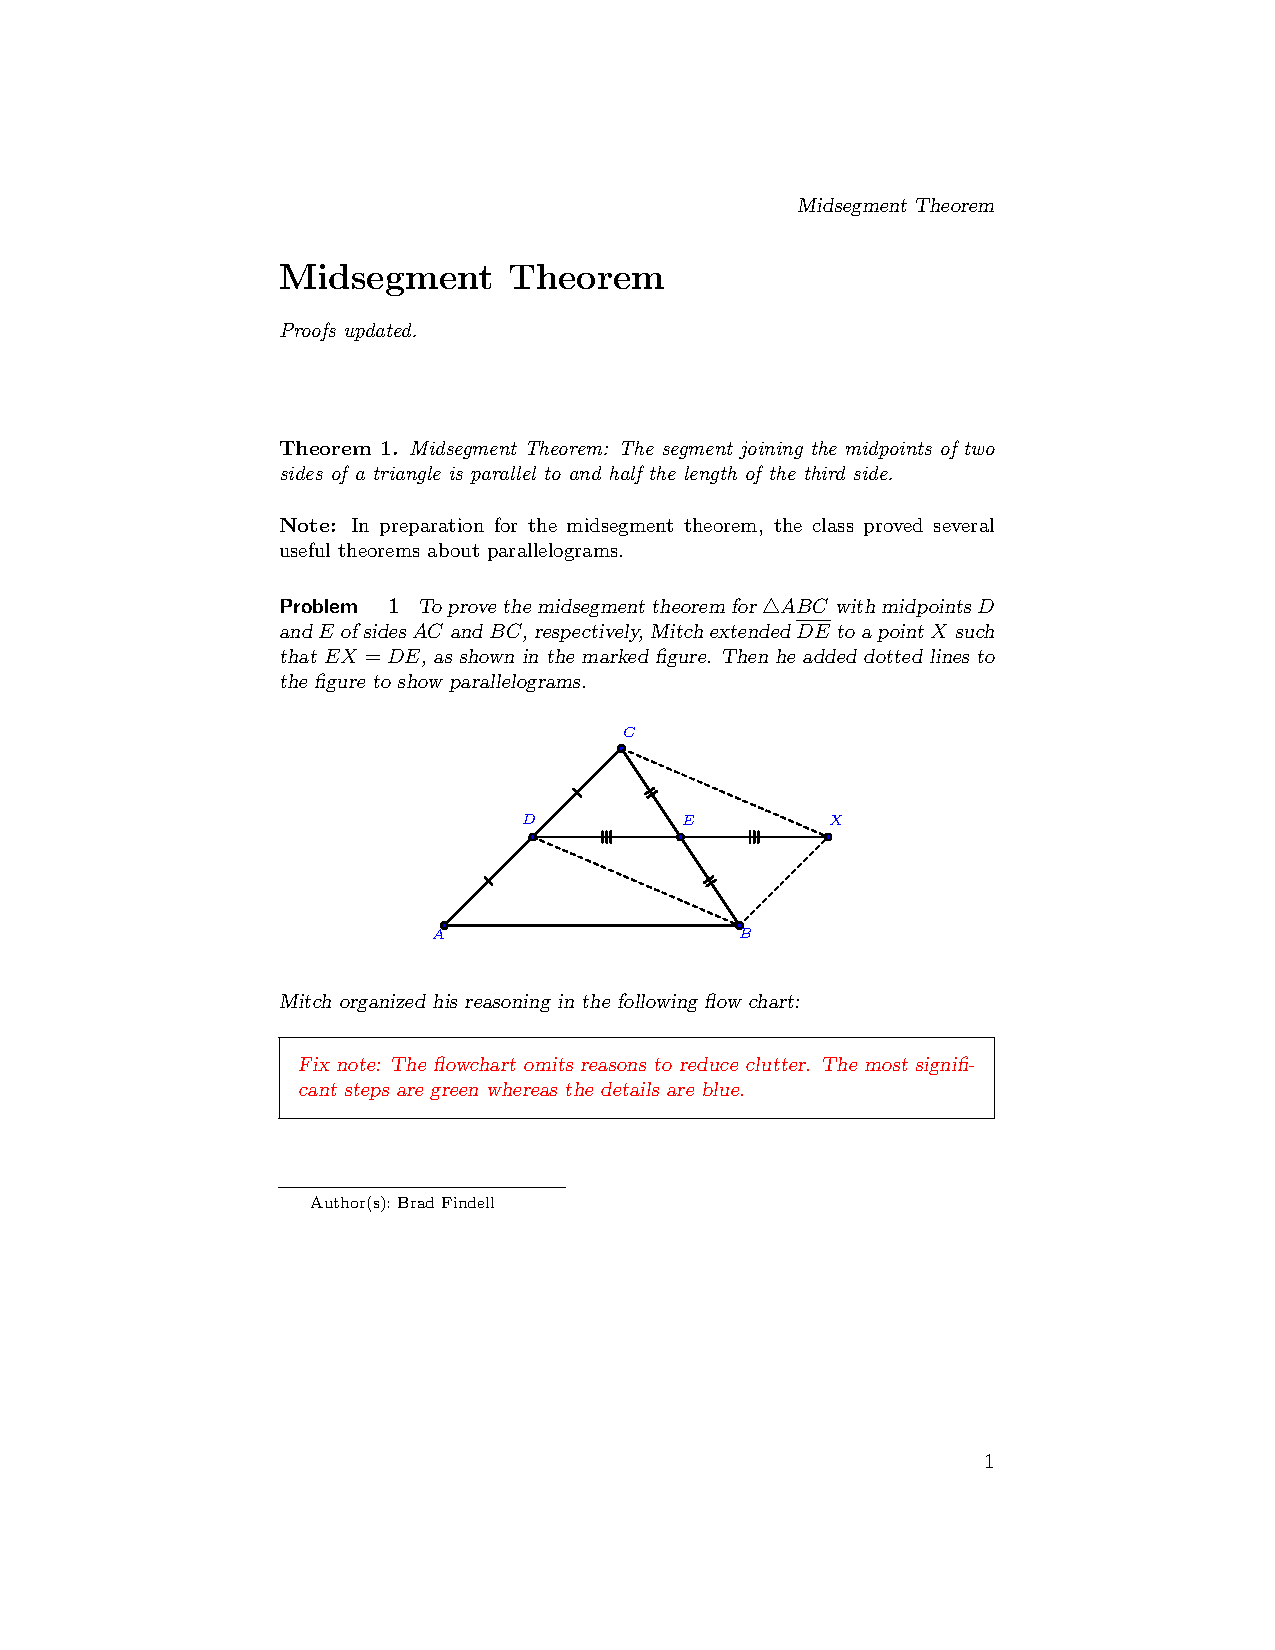
\includegraphics[scale=0.7]{../graphics/midsegment}$$

\begin{image}
\definecolor{qqqqff}{rgb}{0.,0.,1.}
\begin{tikzpicture}[line width=0.8pt,line cap=round,line join=round,>=triangle 45,x=1.0cm,y=1.0cm]
\draw (5.,0.)-- (0.,0.);
\draw (0.,0.)-- (1.5,1.5);
\draw (0.686,0.814) -- (0.814,0.686);
\draw (1.5,1.5)-- (3.,3.);
\draw (2.186,2.314) -- (2.314,2.187);
\draw (1.5,1.5)-- (4.,1.5);
\draw (2.68,1.59) -- (2.68,1.41);
\draw (2.75,1.59) -- (2.75,1.41);
\draw (2.82,1.59) -- (2.82,1.41);
\draw (4.,1.5)-- (6.5,1.5);
\draw (5.18,1.59) -- (5.18,1.41);
\draw (5.25,1.59) -- (5.25,1.41);
\draw (5.32,1.59) -- (5.32,1.41);
\draw (3.,3.)-- (4.,1.5);
\draw (3.555,2.329) -- (3.406,2.229);
\draw (3.594,2.271) -- (3.444,2.171);
\draw (4.,1.5)-- (5.,0.);
\draw (4.555,0.829) -- (4.406,0.729);
\draw (4.594,0.771) -- (4.445,0.671);
\draw [line width=0.6pt,dash pattern=on 2pt off 2pt] (5.,0.)-- (6.5,1.5);
\draw [line width=0.6pt,dash pattern=on 2pt off 2pt] (3.,3.)-- (6.5,1.5);
\draw [line width=0.6pt,dash pattern=on 2pt off 2pt] (1.5,1.5)-- (5.,0.);
\begin{scriptsize}
\draw [fill=qqqqff] (0.,0.) circle (1.5pt);
\draw[color=qqqqff] (-0.1,-0.15) node {$A$};
\draw [fill=qqqqff] (5.,0.) circle (1.5pt);
\draw[color=qqqqff] (5.1,-0.13) node {$B$};
\draw [fill=qqqqff] (3.,3.) circle (1.5pt);
\draw[color=qqqqff] (3.14,3.27) node {$C$};
\draw [fill=qqqqff] (6.5,1.5) circle (1.5pt);
\draw[color=qqqqff] (6.64,1.79) node {$X$};
\draw [fill=qqqqff] (1.5,1.5) circle (1.5pt);
\draw[color=qqqqff] (1.44,1.81) node {$D$};
\draw [fill=qqqqff] (4.,1.5) circle (1.5pt);
\draw[color=qqqqff] (4.14,1.79) node {$E$};
\draw[color=white] (-2.,0.) circle (0.2pt);
\draw[color=white] (8.5,0.) circle (0.2pt);
\end{scriptsize}
\end{tikzpicture}
\end{image}

Mitch organized his reasoning in the following flow chart:  
%\fixnote{The flowchart omits reasons to reduce clutter.  The most significant steps are green whereas the details are blue.}

\begin{image}
\tikzstyle{block} = [rectangle, draw, fill=blue!20, 
    text width=6em, text centered, rounded corners, minimum height=2em]
\tikzstyle{Block} = [rectangle, draw, fill=green!20, 
    text width=10em, text centered, rounded corners, minimum height=3em]
\tikzstyle{implies} = [draw, -latex']

\begin{tikzpicture}[node distance = 1.5cm, auto]
    % Place nodes
    \node [Block] (a) {Quad. $CDBX$ is a parallelogram};
    \node [block, left of=a, node distance = 3.5cm] (init) {$CE = BE$\\$DE=EX$};
    \node [block, below of=a] (b) {$XB=CD$};
    \node [block, left of=b, node distance = 3.5cm] (init2) {$CD=AD$};
    \node [block, below of=b] (c) {$XB=AD$};
    \node [block, right of=b, node distance = 3.5cm] (d) {$\overline{XB} \parallel \overline{CD}$};
    \node [block, below of=d] (e) {$\overline{XB} \parallel \overline{AD}$};
    \node [Block, below of=c] (f) {Quad. $DABX$ is a parallelogram};
    \node [block, below of=f] (g) {$\overline{DX} \parallel \overline{AB}$};
    \node [block, below of=g] (h) {$\overline{DE} \parallel \overline{AB}$};
    \node [block, right of=f, node distance = 3.5cm] (i) {$AB = DX$};
    \node [block, text width=12em, right of=i, node distance = 4cm] (j) {$DX = DE + EX = 2DE$};
    \node [block, below of=i] (k) {$AB = 2DE$};
    \node [block, below of=k] (l) {$DE = \frac{1}{2}AB$};
    \node [Block, text width=12em, below of=h] (m) 
       {Summary: $\overline{DE}$ is parallel to $\overline{AB}$ and half its length.};    
      % Draw edges
    \path [implies] (init) -- (a);
    \path [implies] (a) -- (b);
    \path [implies] (init2) -- (c);
    \path [implies] (b) -- (c);
    \path [implies] (a) -- (d);
    \path [implies] (d) -- (e);
    \path [implies] (c) -- (f);
    \path [implies] (e) -- (f);
    \path [implies] (f) -- (g);
    \path [implies] (g) -- (h);
    \path [implies] (f) -- (i);
    \path [implies] (i) -- (k);
    \path [implies] (j) -- (k);
    \path [implies] (k) -- (l);
    \path [implies] (h) -- (m);
    \path [implies] (l) -- (m);
\end{tikzpicture}
\end{image}

%\fixnote{Is this a helpful way to write the theorems in words? Another approach would be to list them as ``conditions that guarantee a parallelogram.''}

In the proof above, which theorem may Mitch use to conclude that quadrilateral $CDBX$ a parallelogram?  
\begin{multipleChoice}
\choice{If a pair of sides of a quadrilateral are congruent and parallel, then it is a parallelogram.}
\choice[correct]{If the diagonals of a quadrilateral bisect each other, then it is a parallelogram.}
\choice{If opposite sides of a quadrilateral are congruent, then it is a parallelogram.}
\choice{If opposite angles of a quadrilateral are congruent, then it is a parallelogram.}
\choice{The Pythagorean Theorem.}
\choice{None of these.}
\end{multipleChoice}

\begin{problem}
In the proof above, which theorem may Mitch use to conclude that quadrilateral $DABX$ a parallelogram?  
\begin{multipleChoice}
\choice[correct]{If one pair of sides of a quadrilateral are congruent and parallel, then the quadrilateral is a parallelogram.}
\choice{If the diagonals of a quadrilateral bisect each other, then it is a parallelogram.}
\choice{If opposite sides of a quadrilateral are congruent, then it is a parallelogram.}
\choice{If opposite angles of a quadrilateral are congruent, then it is a parallelogram.}
\choice{The Pythagorean Theorem.}
\choice{None of these.}
\end{multipleChoice}

\begin{feedback}[correct]
Here is the proof in a more traditional format: 
\begin{enumerate}
\item $CE = BE$ and $DX=EX$, as given.
\item Quadrilateral $CDBX$ is a parallelogram because the diagonals bisect each other. 
\item $XB=CD$ because opposite sides of a parallelogram are congruent.
\item $XB=AD$ because they are both equal to $CD$. 
\item $\overline{XB} \parallel \overline{CD}$ because $CDBX$ is a parallelogram. 
\item $\overline{XB} \parallel \overline{AD}$ because $A$, $C$, and $D$ are collinear. 
\item Quadrilateral $DABX$ is a parallelogram because a pair of sides is congruent and parallel.  
\item $\overline{DX} \parallel \overline{AB}$ because $DABX$ is a parallelogram. 
\item $\overline{DE} \parallel \overline{AB}$ because $D$, $E$, and $X$ are collinear.  
\item $AB = DX = DE + EX = 2DE$
\item $DE = \frac{1}{2}AB$
\item Summary:  $DE$ is parallel to $AB$ and half its length.  
\end{enumerate}
\end{feedback}
\end{problem}

\end{problem}


\end{document}

